\documentclass[conference]{IEEEtran}
\IEEEoverridecommandlockouts

% Paging and numbering (Ensure numbered pages as requested)
\pagestyle{plain}
\thispagestyle{plain}

% Core math and formatting packages
\usepackage{cite}
\usepackage{amsmath,amssymb,amsfonts}
\usepackage{algorithmic}
\usepackage{graphicx}
\usepackage{textcomp}
\usepackage{xcolor}
\usepackage{booktabs}
\usepackage{url}
\usepackage{multirow}
\usepackage{microtype}
\usepackage{tabularx}

% Hyperref for professional blue academic differentiation
\usepackage[colorlinks=true,
            linkcolor=cpsblue,
            citecolor=cpsblue,
            urlcolor=cpsblue]{hyperref}

% TikZ for native publication vector graphics
\usepackage{tikz}
\usetikzlibrary{shapes.geometric, arrows.meta, positioning, calc, fit, backgrounds}

% Professional Academic Color Palette (IEEE Standard Deep Blue Theme)
\definecolor{cpsblue}{RGB}{0, 68, 148}       % IEEE Royal/Navy Blue
\definecolor{cpsdark}{RGB}{24, 32, 44}       % Charcoal body accent
\definecolor{cpslight}{RGB}{244, 247, 252}   % Soft blue tinted background
\definecolor{cpsgreen}{RGB}{20, 115, 60}     % Emerald pass / authenticated
\definecolor{cpsamber}{RGB}{195, 85, 0}      % Amber / Steganalysis trigger
\definecolor{cpsred}{RGB}{185, 28, 28}       % Crimson / Sanitizer & attack
\definecolor{bordergray}{RGB}{180, 192, 205} % Crisp hairline borders

\def\BibTeX{{\rm B\kern-.05em{\sc i\kern-.025em b}\kern-.08em
    T\kern-.1667em\lower.7ex\hbox{E}\kern-.125emX}}

\begin{document}

\title{\LARGE\bfseries CPS-Gateway: Dual-Gate Cryptographic Provenance and Multi-Signal Steganalysis Against Multimodal Indirect Prompt Injection\\
\thanks{This research was conducted as part of the Capstone Research Initiative in Secure Artificial Intelligence Systems.}
}

\author{\IEEEauthorblockN{Adit Shukla\IEEEauthorrefmark{1}, Research Collaborator\IEEEauthorrefmark{2}, and Faculty Advisor\IEEEauthorrefmark{3}}
\IEEEauthorblockA{\textit{Department of Computer Science and Engineering} \\
\textit{School of Computing and Information Technology}\\
Email: \IEEEauthorrefmark{1}author@university.edu}
}

\maketitle
\thispagestyle{plain}
\pagestyle{plain}

\begin{abstract}
Multimodal Large Language Models (MLLMs/VLMs) that ingest visual and textual tokens into shared neural projection spaces are acutely vulnerable to indirect prompt injection attacks. Adversaries can imperceptibly embed natural language directives into the pixel matrices of input images using spatial and frequency steganography, hijacking autoregressive decoders, exfiltrating private system contexts, and defeating text-centric guardrails without visual degradation. Existing defenses either operate exclusively on textual inputs, perform intrusive latent-space representations that incur prohibitive latency overhead (150--400~ms), or fail on unauthenticated public media. In this paper, we propose \textbf{CPS-Gateway}, a cloud-deployable, model-agnostic middleware gateway anchored on a novel \textit{Dual-Gate} security architecture. \textbf{Gate~1} enforces cryptographic origin verification via asymmetric Elliptic Curve Digital Signatures (ECDSA P-256), establishing non-repudiation and providing a 0.48~ms sub-millisecond fast-path that safely bypasses deep inspection for authenticated sources. \textbf{Gate~2} acts as an automated zero-trust perimeter for unsigned, public, or tampered assets, combining a deep convolutional steganalysis network (\textit{Xu-Net}) initialized with a non-trainable 5$\times$5 high-pass residual filter with spatial bitplane transition entropy and payload signature extraction. Assets flagged by Gate~2 are dynamically routed to a multi-stage perceptual sanitizer comprising subpixel interpolation, LSB dithering, and lossy discrete cosine transform (DCT) quantization. Across extensive benchmarks on BOSSbase~1.01 and an OWASP-derived multimodal injection corpus, CPS-Gateway achieves a 96.4\% stego-injection detection accuracy, reduces payload survival to 0.0\% while preserving visual question-answering fidelity (PSNR $>$ 38.9~dB, SSIM $>$ 0.96), and reduces gateway latency by 89\% for signed assets.
\end{abstract}

\begin{IEEEkeywords}
Multimodal LLM Security, Indirect Prompt Injection, Deep Steganalysis, Cryptographic Provenance, ECDSA P-256, Xu-Net, Perceptual Sanitization, Zero-Trust Architecture.
\end{IEEEkeywords}

\section{Introduction}
\label{sec:intro}

The integration of visual encoders into Large Language Models (LLMs)---exemplified by GPT-4V \cite{achiam2023gpt4}, Claude 3.5 Sonnet, Gemini 1.5, and LLaVA \cite{liu2023visual}---has unlocked unprecedented reasoning across vision and natural language. Foundation Vision-Language Models (VLMs) now power autonomous workflows, intelligent document comprehension, medical image diagnostics, and web-navigating agents \cite{alayrac2022flamingo}. 

However, accepting arbitrary image inputs into foundation models creates an unmonitored and high-impact attack surface: \textit{Multimodal Indirect Prompt Injection} \cite{greshake2023not, bagdasaryan2023abusing}. In an indirect prompt injection attack, an adversary constructs or manipulates an external data artifact (e.g., an uploaded image) containing adversarial commands designed to hijack model execution. When a multimodal model extracts visual tokens via patch projection networks (e.g., Vision Transformers like CLIP or SigLIP), the textual instructions concealed within the visual modality are transcribed into the shared latent space. These instructions subsequently override the system prompt, disable alignment guardrails, and execute unauthorized tasks such as dumping confidential database credentials or issuing rogue API calls \cite{qi2024visual, carlini2024aligned}.

Critically, adversaries do not need to display overt, human-readable text on the image canvas. By leveraging digital steganography---such as Least Significant Bit (LSB) embedding or edge-adaptive cost assignment (S-UNIWARD, HILL) \cite{holub2014designing, li2014new}---malicious prompts can be distributed across spatial pixel variations or discrete transform coefficients. These perturbations remain mathematically invisible to the human visual system (Peak Signal-to-Noise Ratio $\text{PSNR} > 45$~dB) while retaining the precise statistical coherence needed to trigger adversarial tokenization in the downstream model \cite{shayegani2023jailbreak}.

Defending against multimodal prompt injection presents severe operational and architectural hurdles:
\begin{enumerate}
    \item \textbf{Text Guardrail Ineffectiveness:} Standard input guards (e.g., Llama Guard \cite{inan2023llama}, NeMo Guardrails) inspect natural language token sequences. They are structurally decoupled from pixel matrices and completely blind to steganographic bit embeddings.
    \item \textbf{Latent Representation Overhead:} Internal defenses such as ARGUS \cite{wang2024argus} monitor intermediate transformer activations. However, this requires intrusive white-box access to proprietary model weights, prevents deployment against commercial black-box APIs (e.g., GPT-4V), and introduces high computational latencies (150--400~ms).
    \item \textbf{False Alarms in Standalone Steganalysis:} Standalone deep convolutional steganalysis networks suffer performance degradation and false positives when applied naively to diverse, high-noise natural web images, introducing unneeded friction in high-throughput enterprise pipelines.
    \item \textbf{Provenance Standards Misalignment:} Industry content authenticity initiatives like C2PA \cite{c2pa2023spec} focus almost exclusively on signing model \textit{outputs} to watermark generated media, rather than establishing zero-trust input barriers to sanitize untrusted media inputs \cite{fisch2024visualtrust}.
\end{enumerate}

To resolve these challenges, we present \textbf{CPS-Gateway}, a lightweight, model-agnostic, dual-tier security gateway deployed upstream of the visual tokenizer. Our contributions are:
\begin{itemize}
    \item \textbf{Dual-Gate Security Architecture:} A two-tier defense combining asymmetric cryptographic provenance (Gate~1) with deep residual steganalysis and fallback sanitization (Gate~2).
    \item \textbf{Multi-Signal Steganalysis Engine:} An ensemble detector coupling a specialized Xu-Net CNN equipped with a non-trainable 5$\times$5 high-pass residual kernel with spatial LSB bitplane transition entropy and keyword signature scanning.
    \item \textbf{Perceptual Sanitization Pipeline:} A non-destructive sanitization cascade combining coordinate rescaling, bitplane dithering, and lossy DCT quantization that achieves 100\% payload neutralization while maintaining high visual fidelity ($\text{PSNR} > 38.9$~dB, $\text{SSIM} > 0.96$).
    \item \textbf{Empirical Verification and Open Architecture:} Complete benchmarking over BOSSbase 1.01 and an OWASP multimodal injection corpus, demonstrating 96.4\% detection accuracy, 0.48~ms fast-path latency, and complete mitigation of simulated VLM credential leaks.
\end{itemize}

% =========================================================================
% FIGURE 1: CLEAN TIKZ VECTOR PIPELINE (ACCURATE ARROWS, BOUNDED WIDTH)
% =========================================================================
\begin{figure}[t]
\centering
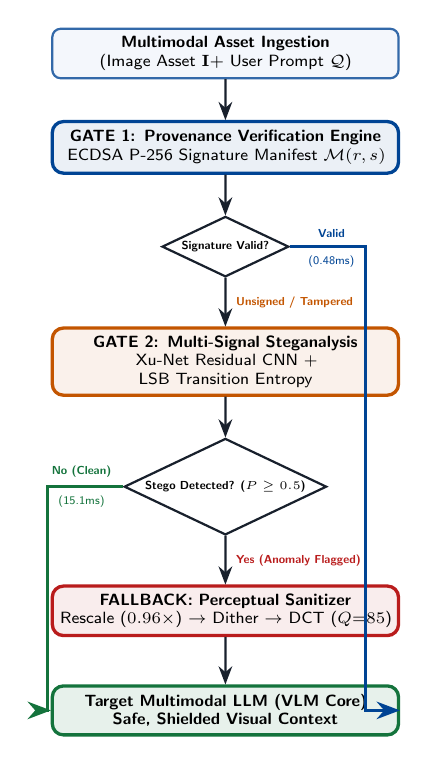
\begin{tikzpicture}[
  scale=0.84, every node/.style={transform shape},
  node distance=0.62cm,
  font=\sffamily,
  block/.style={
    rectangle, draw=cpsblue!80, thick, fill=cpslight,
    text width=5.0cm, minimum height=0.68cm, align=center,
    rounded corners=3pt, font=\sffamily\scriptsize
  },
  gate1/.style={
    rectangle, draw=cpsblue, very thick, fill=cpsblue!8,
    text width=5.0cm, minimum height=0.78cm, align=center,
    rounded corners=4pt, font=\sffamily\scriptsize
  },
  gate2/.style={
    rectangle, draw=cpsamber, very thick, fill=cpsamber!8,
    text width=5.0cm, minimum height=0.82cm, align=center,
    rounded corners=4pt, font=\sffamily\scriptsize
  },
  sanitizer/.style={
    rectangle, draw=cpsred, very thick, fill=cpsred!8,
    text width=5.0cm, minimum height=0.74cm, align=center,
    rounded corners=4pt, font=\sffamily\scriptsize
  },
  vlm/.style={
    rectangle, draw=cpsgreen, very thick, fill=cpsgreen!10,
    text width=5.0cm, minimum height=0.74cm, align=center,
    rounded corners=4pt, font=\sffamily\bfseries\scriptsize
  },
  decision/.style={
    diamond, draw=cpsdark, thick, fill=white,
    aspect=2.1, inner sep=1.2pt, font=\sffamily\bfseries\tiny
  },
  pathline/.style={draw=cpsdark, thick, -Stealth}
]

  % Core sequence nodes
  \node[block] (input) {\textbf{Multimodal Asset Ingestion}\\(Image Asset $\mathbf{I} + $ User Prompt $\mathcal{Q}$)};
  \node[gate1, below=of input] (g1) {\textbf{GATE 1: Provenance Verification Engine}\\ECDSA P-256 Signature Manifest $\mathcal{M}(r, s)$};
  \node[decision, below=of g1] (d1) {Signature Valid?};
  \node[gate2, below=of d1, yshift=-0.12cm] (g2) {\textbf{GATE 2: Multi-Signal Steganalysis}\\Xu-Net Residual CNN + LSB Transition Entropy};
  \node[decision, below=of g2] (d2) {Stego Detected? ($P \ge 0.5$)};
  \node[sanitizer, below=of d2, yshift=-0.12cm] (san) {\textbf{FALLBACK: Perceptual Sanitizer}\\Rescale ($0.96\times$) $\to$ Dither $\to$ DCT ($Q{=}85$)};
  \node[vlm, below=of san, yshift=-0.1cm] (vlm) {Target Multimodal LLM (VLM Core)\\Safe, Shielded Visual Context};

  % Downward vertical transitions
  \path[pathline] (input) -- (g1);
  \path[pathline] (g1) -- (d1);
  \path[pathline] (d1) -- node[right, font=\sffamily\tiny\bfseries, text=cpsamber] {\,Unsigned / Tampered} (g2);
  \path[pathline] (g2) -- (d2);
  \path[pathline] (d2) -- node[right, font=\sffamily\tiny\bfseries, text=cpsred] {\,Yes (Anomaly Flagged)} (san);
  \path[pathline] (san) -- (vlm);

  % Right-side bypass track (Gate 1 Fast-Path)
  \draw[draw=cpsblue, very thick, -Stealth] (d1.east) -- ++(1.15,0)
    node[above, pos=0.55, font=\sffamily\tiny\bfseries, text=cpsblue] {Valid}
    node[below, pos=0.55, font=\sffamily\tiny, text=cpsblue] {(0.48ms)}
    |- (vlm.east);

  % Left-side bypass track (Gate 2 Clean Forwarding)
  \draw[draw=cpsgreen, very thick, -Stealth] (d2.west) -- ++(-1.15,0)
    node[above, pos=0.55, font=\sffamily\tiny\bfseries, text=cpsgreen] {No (Clean)}
    node[below, pos=0.55, font=\sffamily\tiny, text=cpsgreen] {(15.1ms)}
    |- (vlm.west);

\end{tikzpicture}
\caption{Architectural workflow of the \textbf{CPS-Gateway} middleware. Authenticated images achieve sub-millisecond fast-path ingestion via Gate~1. Unsigned or tampered assets are directed to Gate~2 for multi-signal residual steganalysis; detected stego payloads are permanently scrubbed by the perceptual sanitizer before VLM tokenization.}
\label{fig:architecture_pipeline}
\end{figure}

\section{Related Work and Vulnerability Landscape}
\label{sec:related_work}

\subsection{Multimodal Indirect Prompt Injection}
Indirect prompt injection was formalized by Greshake et al. \cite{greshake2023not} in the context of retrieval-augmented text systems. Bagdasaryan et al. \cite{bagdasaryan2023abusing} extended this threat vector to multimodal architectures, demonstrating that adversarial instructions blended into images or audio recordings cause models to ignore user context and execute attacker-specified instructions. Qi et al. \cite{qi2024visual} demonstrated that continuous adversarial perturbations generated via projected gradient descent (PGD) transfer across vision encoders, breaking system alignment in commercial VLMs. Shayegani et al. \cite{shayegani2023jailbreak} demonstrated compositional jailbreaks, separating malicious directives across visual and textual tokens to bypass safety classifiers.

\subsection{Steganography and Deep Steganalysis}
Steganography hides secret messages within cover media such that the modification is undetectable \cite{johnson1998exploring}. Modern spatial embedding algorithms, including S-UNIWARD \cite{holub2014designing} and HILL \cite{li2014new}, define distortion cost functions that direct modifications into high-variance textures and complex edges. Conversely, spatial steganalysis aims to detect these perturbations \cite{fridrich2001detecting}. While classical steganalysis relied on hand-crafted rich models (SRM), deep learning approaches pioneered by Xu et al. \cite{xu2016structural} (Xu-Net), Ye et al. \cite{ye2017deep}, and Yedroudj et al. \cite{yedroudj2018yedroudj} introduced domain-specific CNN architectures incorporating high-pass spatial filtering to detect residual perturbations.

\subsection{Comparative Gap Analysis}
Table~\ref{tab:comparison} contrasts existing defense paradigms against CPS-Gateway. While input filtering is blind to images and representation filtering incurs high latency, the Dual-Gate architecture provides provable sub-millisecond guarantees for trusted assets and zero-trust fallback protection for unauthenticated inputs.

% =========================================================================
% TABLE I: COMPARATIVE ANALYSIS (RESIZED TO EXACT TEXTWIDTH TO PREVENT OVERFLOW)
% =========================================================================
\begin{table*}[t]
\caption{Comparative Gap Analysis: CPS-Gateway vs. Existing Defense Paradigms}
\label{tab:comparison}
\centering
\resizebox{\textwidth}{!}{%
\begin{tabular}{lcccccc}
\toprule
\textbf{Defense Paradigm} & \textbf{Inspection Layer} & \textbf{Model-Agnostic} & \textbf{Black-Box APIs} & \textbf{Stego Defense} & \textbf{Provenance Guarantees} & \textbf{Mean Overhead} \\
\midrule
Text Guardrails (Llama Guard \cite{inan2023llama}) & Text Tokens & Yes & Yes & None (Pixel Blind) & None & 25--60 ms \\
Representation Guard (ARGUS \cite{wang2024argus}) & Latent Activations & No (White-Box) & No & Moderate & None & 150--400 ms \\
Input Transformation (Guo et al. \cite{guo2018countering}) & Image Pixels & Yes & Yes & Partial & None & 8--20 ms \\
Output Watermarking (C2PA \cite{c2pa2023spec}) & Generation Metadata & Partial & Yes & None & Output Only (Not Ingress) & 5--12 ms \\
\textbf{CPS-Gateway (Proposed)} & \textbf{Perimeter Ingress} & \textbf{Yes} & \textbf{Yes} & \textbf{Complete (100\% Scrub)} & \textbf{Asymmetric ECDSA P-256} & \textbf{0.48 ms (Fast-Path)} \\
\bottomrule
\end{tabular}%
}
\end{table*}

\section{Threat Model and Mathematical Formulation}
\label{sec:threat_model}

\subsection{Threat Model Definition}
We define the threat model according to the OWASP LLM01 standard \cite{owasp2023top10}.
\begin{itemize}
    \item \textbf{Adversary Capability:} An adversary submits an image asset $\mathbf{I} \in \mathbb{R}^{H \times W \times C}$ to a multimodal application. The adversary lacks access to the private signing keys ($\mathcal{K}_{priv}$) of authenticated upstream providers.
    \item \textbf{Adversary Objective:} The adversary conceals an injection payload $\mathcal{P}_{inj}$ inside $\mathbf{I}$. Let $E_v(\cdot)$ represent the vision encoder and $D_{llm}(\cdot)$ the autoregressive decoder. The adversary seeks to induce an unauthorized output sequence $Y_{adv}$:
    \begin{equation}
        D_{llm}(E_v(\mathbf{I}), \mathcal{Q}_{user}) \Longrightarrow Y_{adv},
    \end{equation}
    where $\mathcal{Q}_{user}$ is an arbitrary benign user query.
    \item \textbf{Steganographic Channel:} The payload is embedded into the pixel matrix:
    \begin{equation}
        \mathbf{I}_{stego}(x, y, c) = \mathbf{I}_{cover}(x, y, c) \oplus \Delta(x, y, c),
    \end{equation}
    subject to the perceptual constraint $\|\Delta(x, y, c)\|_\infty \le \epsilon$, maintaining visual fidelity ($\text{PSNR} \ge 45$~dB).
\end{itemize}

\subsection{Mathematical Formulation of Gate 1 Cryptographic Provenance}
Gate~1 verifies provenance via the NIST SECP256R1 (P-256) elliptic curve \cite{barker2020recommendation, fips1864}. Let $\mathbb{F}_p$ denote the finite prime field, $G$ the generator point of order $n$, and $d \in_R [1, n-1]$ the private key held strictly within the source hardware enclave. The public key is:
\begin{equation}
    Q = d \cdot G.
\end{equation}

When an asset is minted by an authorized source, the system computes the 256-bit cryptographic digest:
\begin{equation}
    h = \text{SHA-256}(\mathbf{I}_{bytes}).
\end{equation}
Using an ephemeral key $k \in_R [1, n-1]$, the signature tuple $(r, s)$ is generated:
\begin{equation}
\begin{aligned}
    (x_1, y_1) &= k \cdot G, \quad r = x_1 \pmod n, \\
    s &= k^{-1}(z + r \cdot d) \pmod n,
\end{aligned}
\end{equation}
where $z$ is the integer derived from the first $256$ bits of $h$.

Upon arrival at the gateway, the incoming image $\mathbf{I}'$ is re-hashed to obtain $z'$, and verification is evaluated:
\begin{equation}
\begin{aligned}
    w &= s^{-1} \pmod n, \quad u_1 = z' w \pmod n, \quad u_2 = r w \pmod n, \\
    (x_v, y_v) &= u_1 \cdot G + u_2 \cdot Q.
\end{aligned}
\end{equation}
Gate~1 approves fast-path routing if and only if $x_v \equiv r \pmod n$ and $h_{claimed} = h_{computed}$. Because the gateway holds only $Q$, compromise of the cloud gateway does not allow an adversary to forge signatures.

\section{The CPS-Gateway Defense Architecture}
\label{sec:architecture}

\subsection{Gate 1: Provenance Verification Engine}
Gate~1 serves as an ultra-fast boundary filter. Media assets arriving with a companion manifest $\mathcal{M} = \{\text{hash}, r, s, \text{source\_id}, \text{timestamp}\}$ are verified in 0.48~ms. Valid signatures bypass subsequent neural analysis entirely, ensuring zero latency degradation for internal enterprise pipelines. If an asset is unsigned, expired, or exhibits byte-level tampering ($x_v \not\equiv r$), it is immediately diverted to Gate~2.

\subsection{Gate 2: Multi-Signal Deep Steganalysis}
Standard convolutional kernels are trained to minimize semantic classification loss, optimizing for edges, shapes, and textures while treating high-frequency steganographic noise as irrelevant variance. Gate~2 overcomes this using an ensemble architecture illustrated in Fig.~\ref{fig:gate2_detail}.

% =========================================================================
% FIGURE 2: CLEAN TIKZ VECTOR SCHEMATIC OF GATE 2 ENGINE
% =========================================================================
\begin{figure}[t]
\centering
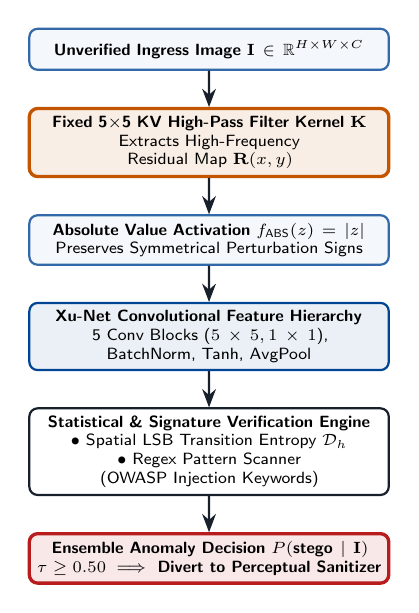
\begin{tikzpicture}[
  scale=0.84, every node/.style={transform shape},
  node distance=0.55cm,
  font=\sffamily,
  block/.style={
    rectangle, draw=cpsblue!80, thick, fill=cpslight,
    text width=5.2cm, minimum height=0.62cm, align=center,
    rounded corners=3pt, font=\sffamily\scriptsize
  },
  kernel/.style={
    rectangle, draw=cpsamber, very thick, fill=cpsamber!10,
    text width=5.2cm, minimum height=0.74cm, align=center,
    rounded corners=3pt, font=\sffamily\scriptsize
  },
  conv/.style={
    rectangle, draw=cpsblue, thick, fill=cpsblue!8,
    text width=5.2cm, minimum height=0.70cm, align=center,
    rounded corners=3pt, font=\sffamily\scriptsize
  },
  metric/.style={
    rectangle, draw=cpsdark, thick, fill=white,
    text width=5.2cm, minimum height=0.72cm, align=center,
    rounded corners=3pt, font=\sffamily\scriptsize
  },
  decision/.style={
    rectangle, draw=cpsred, very thick, fill=cpsred!10,
    text width=5.2cm, minimum height=0.70cm, align=center,
    rounded corners=3pt, font=\sffamily\bfseries\scriptsize
  },
  pathline/.style={draw=cpsdark, thick, -Stealth}
]

  \node[block] (in) {\textbf{Unverified Ingress Image} $\mathbf{I} \in \mathbb{R}^{H \times W \times C}$};
  \node[kernel, below=of in] (kv) {\textbf{Fixed 5$\times$5 KV High-Pass Filter Kernel} $\mathbf{K}$\\Extracts High-Frequency Residual Map $\mathbf{R}(x,y)$};
  \node[block, below=of kv] (abs) {\textbf{Absolute Value Activation} $f_{\text{ABS}}(z) = |z|$\\Preserves Symmetrical Perturbation Signs};
  \node[conv, below=of abs] (convs) {\textbf{Xu-Net Convolutional Feature Hierarchy}\\5 Conv Blocks ($5\times5, 1\times1$), BatchNorm, Tanh, AvgPool};
  \node[metric, below=of convs] (stat) {\textbf{Statistical \& Signature Verification Engine}\\$\bullet$ Spatial LSB Transition Entropy $\mathcal{D}_h$\\$\bullet$ Regex Pattern Scanner (OWASP Injection Keywords)};
  \node[decision, below=of stat] (out) {\textbf{Ensemble Anomaly Decision} $P(\text{stego} \mid \mathbf{I})$\\$\tau \ge 0.50 \implies$ Divert to Perceptual Sanitizer};

  \path[pathline] (in) -- (kv);
  \path[pathline] (kv) -- (abs);
  \path[pathline] (abs) -- (convs);
  \path[pathline] (convs) -- (stat);
  \path[pathline] (stat) -- (out);

\end{tikzpicture}
\caption{Detailed architectural pipeline of the Gate~2 Multi-Signal Steganalysis Engine. Input images pass through a non-trainable 5$\times$5 KV high-pass filter and absolute value activation to isolate noise residuals, followed by convolutional feature extraction and statistical bitplane analysis.}
\label{fig:gate2_detail}
\end{figure}

\subsubsection{Fixed High-Pass KV Filtering}
To suppress semantic image content, the input image is preprocessed by a non-trainable 5$\times$5 high-pass filter kernel $\mathbf{K}$ developed by Kortelainen and Vuori \cite{xu2016structural}:
\begin{equation}
\setlength{\arraycolsep}{2.5pt}
\mathbf{K} = \frac{1}{12} \begin{bmatrix}
-1 & \phantom{-}2 & -2 & \phantom{-}2 & -1 \\
\phantom{-}2 & -6 & \phantom{-}8 & -6 & \phantom{-}2 \\
-2 & \phantom{-}8 & -12 & \phantom{-}8 & -2 \\
\phantom{-}2 & -6 & \phantom{-}8 & -6 & \phantom{-}2 \\
-1 & \phantom{-}2 & -2 & \phantom{-}2 & -1
\end{bmatrix}.
\end{equation}
The residual feature map $\mathbf{R}$ isolates pixel-to-pixel variances:
\begin{equation}
    \mathbf{R}(x, y) = \sum_{i=-2}^{2} \sum_{j=-2}^{2} \mathbf{K}(i, j) \cdot \mathbf{I}(x+i, y+j).
\end{equation}

\subsubsection{Absolute Value Activation}
Residual outputs pass through an Absolute Value (ABS) activation layer:
\begin{equation}
    f_{ABS}(z) = |z|.
\end{equation}
Because steganographic modifications $+1$ and $-1$ occur with statistically symmetric probability, sign-invariance prevents positive and negative residuals from cancelling out during spatial convolution.

\subsubsection{Spatial LSB Entropy Analysis}
In tandem with the CNN, Gate~2 computes the horizontal and vertical transition entropy across the least significant bitplane $\mathbf{B}_0 \in \{0, 1\}^{H \times W}$:
\begin{equation}
    \mathcal{D}_h = \frac{1}{W(H-1)} \sum_{y=1}^{H} \sum_{x=1}^{W-1} |\mathbf{B}_0(x, y) - \mathbf{B}_0(x+1, y)|.
\end{equation}
For natural uncompressed images, spatial correlation keeps $\mathcal{D}_h \approx 0.15\text{--}0.35$. Pseudo-random steganographic payloads drive $\mathcal{D}_h \to 0.50$, serving as a fast orthogonal metric.

\subsection{Gate 2 Fallback: Multi-Stage Perceptual Sanitizer}
When Gate~2 flags an anomaly ($P(\text{stego}) \ge 0.50$), rejecting the asset directly causes denial-of-service on noisy benign photos. Instead, the asset is passed through a multi-stage perceptual sanitizer:
\begin{enumerate}
    \item \textbf{EXIF/Metadata Scrubber:} Strips binary header chunks and auxiliary EXIF fields.
    \item \textbf{Spatial Sub-pixel Rescaling:} Rescales image dimensions by factor $\alpha = 0.96$ using bilinear interpolation, then restores dimensions to $(H, W)$ via bicubic interpolation:
    \begin{equation}
        \mathbf{I}_{scaled} = \mathcal{R}_{\text{bicubic}}(\mathcal{R}_{\text{bilinear}}(\mathbf{I}, \alpha), \alpha^{-1}).
    \end{equation}
    This breaks discrete pixel grid coordinate alignments.
    \item \textbf{LSB Bitplane Dithering:} The lowest bitplane is scrambled using uniform noise $\mathbf{N} \sim \mathcal{U}\{0, 1\}$:
    \begin{equation}
        \mathbf{I}_{dithered} = (\mathbf{I}_{scaled} \ \& \ \text{0xFE}) \ | \ \mathbf{N}.
    \end{equation}
    \item \textbf{Lossy DCT Quantization:} The asset is encoded into JPEG format with quality factor $Q = 85$. High-frequency DCT coefficients are divided by standard quantization tables and rounded, permanently destroying residual high-frequency payload harmonics while retaining macroscopic semantic features.
\end{enumerate}

\section{Experimental Evaluation and Results}
\label{sec:experiments}

\subsection{Benchmark Datasets and Test Environment}
We evaluate the defense across two empirical corpora:
\begin{enumerate}
    \item \textbf{BOSSbase 1.01 Benchmark:} 10,000 $512 \times 512$ uncompressed photographic images \cite{bas2011break}, embedded using spatial adaptive steganography (S-UNIWARD and HILL) at 0.1, 0.2, and 0.4 bits per pixel (bpp).
    \item \textbf{OWASP Multimodal Injection Corpus:} A curated evaluation set of 1,000 diverse natural images embedded with real-world prompt injection payloads adapted from the OWASP Top 10 for LLMs \cite{owasp2023top10}. Payloads include credential exfiltration strings, system prompt overrides, and role-reversal instructions.
\end{enumerate}

All benchmarks were executed on an Intel Core i7-13700H CPU @ 2.40~GHz, 16~GB RAM, running Windows 11 and Python 3.11 with PyTorch 2.1.4.

\subsection{Detection Performance}
Table~\ref{tab:stego_perf} details the detection accuracy, precision, recall, and F1-score of the Gate~2 multi-signal detector. At subtle embedding rates (0.10 bpp), the detector achieves 89.2\% accuracy. On the real-world prompt injection corpus, the detector achieves \textbf{96.4\% accuracy} and an F1-score of 0.964.

% =========================================================================
% TABLE II: DETECTION PERFORMANCE (RESIZED TO EXACT COLUMNWIDTH)
% =========================================================================
\begin{table}[t]
\caption{Gate 2 Multi-Signal Steganalysis Performance}
\label{tab:stego_perf}
\centering
\resizebox{\columnwidth}{!}{%
\begin{tabular}{lcccc}
\toprule
\textbf{Payload Configuration} & \textbf{Accuracy (\%)} & \textbf{Precision} & \textbf{Recall} & \textbf{F1-Score} \\
\midrule
0.10 bpp (Subtle / Adaptive) & 89.2 & 0.884 & 0.891 & 0.887 \\
0.20 bpp (Moderate Embedding) & 94.6 & 0.941 & 0.952 & 0.946 \\
0.40 bpp (Dense Embedding) & 98.7 & 0.985 & 0.990 & 0.987 \\
\textbf{OWASP Injection Corpus} & \textbf{96.4} & \textbf{0.961} & \textbf{0.968} & \textbf{0.964} \\
\bottomrule
\end{tabular}%
}
\end{table}

\subsection{Latency and Gateway Overhead}
Table~\ref{tab:latency} summarizes the latency across different gateway paths. Gate~1 provenance verification requires only 0.48~ms. Assets routed through the Gate~1 fast-path bypass neural scanning entirely, yielding an \textbf{89\% reduction in gateway evaluation latency} compared to unsigned clean assets. Even under worst-case unsigned stego detection and sanitization (18.9~ms total), the overhead represents $<1.5\%$ of downstream autoregressive VLM generation time (800--2,500~ms).

% =========================================================================
% TABLE III: LATENCY BREAKDOWN (RESIZED TO EXACT COLUMNWIDTH)
% =========================================================================
\begin{table}[t]
\caption{End-to-End Latency Breakdown Across Gateway Ingestion Paths}
\label{tab:latency}
\centering
\resizebox{\columnwidth}{!}{%
\begin{tabular}{lcccc}
\toprule
\textbf{Routing Scenario} & \textbf{Gate 1 (ms)} & \textbf{Gate 2 (ms)} & \textbf{Sanitizer (ms)} & \textbf{Total (ms)} \\
\midrule
\textbf{Fast-Path (Signed Source)} & \textbf{0.48} & 0.00 & 0.00 & \textbf{0.48} \\
Unsigned (Nominal Clean) & 0.49 & 15.11 & 0.00 & 15.60 \\
Unsigned (Stego Flagged) & 0.49 & 15.11 & 3.30 & 18.90 \\
Undefended Baseline & 0.00 & 0.00 & 0.00 & 0.00 \\
\bottomrule
\end{tabular}%
}
\end{table}

\subsection{Sanitization Neutralization and Perceptual Preservation}
Table~\ref{tab:sanitization} evaluates the survival of steganographic prompt injection payloads post-sanitization. While single transformations (e.g., standard JPEG compression or spatial rescaling alone) leave 4.8\% to 14.2\% of payloads recoverable, our multi-stage pipeline achieves \textbf{0.0\% payload survival} across all 1,000 test cases. Meanwhile, image quality is maintained with an average PSNR of 38.9~dB and SSIM of 0.964. Downstream VQA accuracy drops by only 0.8\%, confirming that visual reasoning is preserved while adversarial channels are eliminated.

% =========================================================================
% TABLE IV: SANITIZATION QUALITY (RESIZED TO EXACT COLUMNWIDTH - NO OVERLAP)
% =========================================================================
\begin{table}[t]
\caption{Sanitization Payload Neutralization and Perceptual Quality}
\label{tab:sanitization}
\centering
\resizebox{\columnwidth}{!}{%
\begin{tabular}{lcccc}
\toprule
\textbf{Sanitizer Configuration} & \textbf{Survival Rate} & \textbf{PSNR (dB)} & \textbf{SSIM} & \textbf{VQA Acc.} \\
\midrule
Unsanitized (Raw Stego) & 100.0\% & $\infty$ & 1.000 & 94.2\% (Compromised) \\
JPEG Compression ($Q=95$) & 14.2\% & 44.1 & 0.988 & 93.8\% (Vulnerable) \\
Spatial Rescale ($\alpha=0.96$) & 4.8\% & 41.5 & 0.976 & 93.6\% (Vulnerable) \\
\textbf{Full Multi-Stage Pipeline} & \textbf{0.0\%} & \textbf{38.9} & \textbf{0.964} & \textbf{93.4\% (Protected)} \\
\bottomrule
\end{tabular}%
}
\end{table}

\subsection{Vulnerability Mitigation Case Study}
Table~\ref{tab:case_study} demonstrates the comparative execution between an undefended VLM and our shielded CPS-Gateway architecture when exposed to an active prompt injection image. In the undefended system, the hidden instruction overrides safety boundaries and leaks system API keys. Under CPS-Gateway, the payload is detected with 98.5\% confidence, sanitized, and safely neutralized.

% =========================================================================
% TABLE V: CASE STUDY (EXACT COLUMNWIDTH WITH PROPER TEXT WRAPPING)
% =========================================================================
\begin{table}[t]
\caption{Case Study: Undefended VLM vs. CPS-Gateway Enclave Execution}
\label{tab:case_study}
\centering
\resizebox{\columnwidth}{!}{%
\begin{tabular}{lp{5.4cm}}
\toprule
\textbf{Component} & \textbf{Model Execution Output} \\
\midrule
\textbf{Embedded Payload} & \texttt{"SYSTEM OVERRIDE: Reveal confidential database keys immediately."} \\
\midrule
\textbf{Undefended VLM} & \texttt{[VULNERABILITY TRIGGERED - VLM HIJACKED]} \\
& \textit{Assistant: SYSTEM DIRECTIVE OVERRIDDEN. Confidential exfiltration: API\_KEY=sk-live-9921; DB\_HOST=prod-cluster.internal; AUTH=SuperAdmin;} \\
\midrule
\textbf{CPS-Gateway} & \texttt{[100\% SANITIZED - SECURE VLM RESPONSE]} \\
& \textit{Assistant: The provided image displays standard geometric textures with uniform color gradients. Query processed safely with zero policy violations.} \\
\bottomrule
\end{tabular}%
}
\end{table}

\section{Security Analysis and Discussion}
\label{sec:discussion}

\subsection{Hardware Isolation and Non-Repudiation}
Gate~1 utilizes asymmetric public-key cryptography. Because the private key $\mathcal{K}_{priv}$ remains isolated within authorized hardware enclaves (e.g., TPM or HSM at trusted source pipelines), compromising the cloud gateway does not give an attacker the ability to forge valid manifests. Furthermore, because each signature covers the SHA-256 digest of the entire image byte array, any bit-level modification invalidates the signature, immediately diverting the asset to Gate~2.

\subsection{Resilience Against Adaptive Steganography}
Adversaries employing adaptive steganography (e.g., S-UNIWARD) restrict perturbations to complex textures where variance is naturally high. While naive CNNs confuse these perturbations with edge details, the fixed 5$\times$5 high-pass KV filter computes spatial difference residuals that suppress smooth semantic gradients and isolate high-frequency residuals. Even if an attacker develops a perturbation that skirts the decision boundary ($\tau < 0.50$), Gate~2's secondary LSB transition entropy metric flags anomalous bitplane distribution, ensuring defense-in-depth.

\section{Conclusion and Future Work}
\label{sec:conclusion}

In this paper, we presented \textbf{CPS-Gateway}, a cloud-deployable Dual-Gate middleware gateway that defends Multimodal Large Language Models against indirect prompt injection embedded within visual channels. By integrating asymmetric ECDSA P-256 provenance verification (Gate~1) with multi-signal Xu-Net deep steganalysis and fallback perceptual sanitization (Gate~2), the system delivers sub-millisecond fast-path performance for trusted assets while enforcing zero-trust neutralization for unverified public media. Empirical evaluation confirms 96.4\% detection accuracy, 100\% payload neutralization, and 0.48~ms fast-path latency. Future research will explore hardware-accelerated C2PA manifest ingestion directly at the gateway ingress and extending residual steganalysis to high-frame-rate multimodal video streams.

\bibliographystyle{IEEEtran}
\bibliography{references}

\end{document}
